\chapter{Introduction}

\section{DDoS}

\section{Botnet}

A botnet is a network of internet-connected devices, such as computers, smartphones or IoT devices, whose security has been compromised and control has been taken over by a third party. 
Botnets were initially designed for legitimate purposes, such as automating repetitive tasks or managing chatrooms. However, their ability to execute code within other computers led to their misuse for malicious activities, such as stealing passwords, tracking user keystrokes, and launching attacks against unsuspecting devices. \cite{fortinet-botnet} They are one of the most common types of \textbf{network-based attacks} today due to their use of large, coordinated groups of hosts. These groups are created by infecting vulnerable hosts,  turning them into ``\textit{zombies}'' or \textbf{bots}, which can then be controlled remotely. When a collection of bots is managed by a \textbf{Command and Control} (CNC) infrastructure, it forms a botnet. Botnets help in obscuring the identity of the attacking host by providing a layer of indirection, separating the attacking host from its victim through zombie hosts, and separating the attack itself from the botnet assembly by an arbitrary amount of time. \cite{strayer2008botnet} The method of controlling bots varies based on the architecture of the botnet's command and control mechanisms, which can be \textbf{Internet Relay Chat} (IRC), \textbf{HTTP}, \textbf{DNS}, or \textbf{P2P-based}. 

\section{Mirai}

Mirai is a malware that targets \textbf{IoT devices}, such as routers, cameras and others, by exploiting their default credentials. Once a device is compromised by Mirai, it becomes part of a botnet that can be used to launch \textbf{DDoS attacks}, however, this do not compromise the device's functionality except for occasional increased bandwidth usage. It is capable of running on various CPU architectures, including MIPS, ARM, and PPC. It uses a dictionary attack with a set of 62 entries to gain control of vulnerable devices. The infected devices are reported to a control server to become part of a large-scale Agent-Handler botnet. \cite{de2018ddos}

The botnet was first created by a guy named Paras Jha, who used it to launch multiple DDoS attacks against Minecraft servers. This was to extort money from the server owners, who would pay him to gain ``protection'' from the attacks. Then it was also used to attack Rutgers University, where he was a student. After these events, he joined forces with other two individuals, Josiah White and Dalton Norman, to further develop the malware, which later became known as Mirai. The malware was first discovered by MalwareMustDie, a non-profit security research group, in August 2016. In the late september of the same year, it gained public attention after being used in a DDoS attack against the Krebs On Security website, reaching 620 Gbps. Following this, it was employed in an attack on the French hosting company OVH, which peaked at 1 Tbps. After these attacks, Anna-senpai, which seems to be the online nickname of Paras Jha, released the source code of Mirai on HackForums\footnote{Original post: \url{https://hackforums.net/showthread.php?tid=5420472}}. This led to the proliferation of Mirai-based botnets and some time later caused the Dyn DDoS attack, which took down several high-profile websites, such as GitHub, Twitter, Reddit, and Netflix. Dyn estimated that up to 100,000 malicious endpoints were involved in the attack. \cite{8115504}

\subsection{Mirai architecture}

The architecture of Mirai is illustraded in \Cref{fig:mirai-architecture} and is based on a \textbf{centrlized} model. The botnet is composed of four main components: 

\begin{itemize}
    \item \textbf{CNC server}: the central component of the botnet, it is used by the admin / users to control the bots and to send commands to them.
    \item \textbf{Bots}: the infected devices that are part of the botnet and are used to launch DDoS attacks. Other than waiting for commands to perform attacks, each bot performs some tasks:
    \begin{itemize}
        \item \textbf{Scanner}: perform active scanning of the internet for vulnerable devices, once found it reports them to the report server. When a device is found it tries to remotely access by using a dictionary based attack with a set of 62 entries. If the attack is successful, the bot will send the vilnerability to the reporting server.
        \item \textbf{Killer}: tries to kill other malware running on the device.
        \item \textbf{Masking}: once the malware is running, it deletes itself from the device to go unnoticed.
    \end{itemize}
    \item \textbf{Reporting server}: its role is to receive the vulnerablity (IP, port and potential username and password) found by the bots and forward them to the loader. 
    \item \textbf{Loader server}: it is in charge of loading the malware on the reported devices. 
\end{itemize}

To summarize, Mirai uses a spreading model named ``Real Time Loading'', which is based on the following steps: Bots $\rightarrow$ Reporting server $\rightarrow$ Loader server $\rightarrow$ Bots. \cite{de2018ddos} More information on how the components works with some code snippets can be found in \Cref{chapter:mirai-static-analysis}.


\begin{figure}[ht]
    \centering
    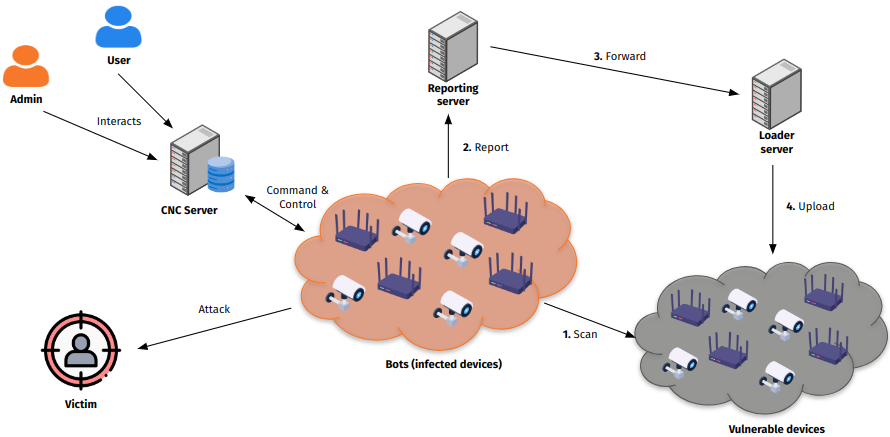
\includegraphics[scale=0.5]{resources/images/mirai-architecture.png}
    \caption{Mirai architecture}
    \label{fig:mirai-architecture}
\end{figure}